\chapter{Background}

In this chapter, we go over some of the background literature related to our study. In \secref{sec:MWE}, we discuss what multiword expressions are and why they pose an interesting problem. \secref{sec:Comp} covers the existing approaches used to predict their compositionality. We then provide a detailed account of various language embedding models in \secref{sec:emb}, as well as their usage in popular NLP tasks.
%Finally, \secref{sec:MTL} looks at a relatively new approach in Machine Learning -- Multi-task Learning.

\section{Multiword Expressions}
\label{sec:MWE}
Multiword expressions, according to \cite{Baldwin2009}, are ``lexical items that (a) can be decomposed into multiple lexemes; and (b) display lexical, syntactic, semantic, pragmatic and/or statistical idiomaticity.'' Some examples of MWEs are \textit{silver screen}, \textit{sure shot} and \textit{a piece of cake}. There are various types of MWEs with various lexical and semantic characteristics. In this study, we focus on noun compounds (NCs) predominantly, but also study adjective-noun phrases (ADJ-NNs):
\begin{itemize}
    \item \textbf{Noun Compounds} Noun compounds (NCs) are MWEs composed solely of nouns. These are commonly observed as binary noun compounds in the English language, wherein the first and second nouns are known as the \textit{modifier} and \textit{head}, respectively. Consider the example of a \textit{student loan}-- the head \textit{loan} conveys the main meaning (i.e. it is a kind of loan), while the modifier \textit{student} tells us specifically what kind of loan it is (a student loan, as opposed to a car loan, say). No NC is truly fully compositional, since its components convey some implicit information together, the nature of which determines their semantic relationship. For example, \textit{breakfast juice} is juice meant for consumption at breakfast versus \textit{orange juice} is juice made from oranges.
    
    \item \textbf{Adjective-Noun Combinations} An adjective-noun (ADJ-NN) pair is a binary MWE that contains a noun preceded by an adjective that describes it. Some examples are \textit{poor man, old school} and \textit{heavy rain}.
\end{itemize}

In this study, we are concerned with the semantic compositionality of these expressions, or the degree to which the meaning of the MWE can be derived from that of its constituents. For example \textit{crocodile tears} is not compositional as it is used in a figurative sense to mean an insincere display of emotion. \textit{Application form}, on the other hand, is highly compositional.

\section{Compositionality Prediction}
\label{sec:Comp}
Most of the early studies of compositionality posed it as a binary classification of compositional/non-compositional \citep{Bannard2003,Bannard2006,Farah2015}, sometimes adding a (third) semi-compositional category. Some studies also consider it to be a regression problem, covering a range of continuous compositionality scores \citep{Baldwin2010,Reddy2011,Salehi2015,Hakimi2018}. The compositionality itself is a prediction of either the MWE on the whole \citep{Mccarthy2003,venkat2005,Disco2011,Kat2015,Farah2015}, relative to each of its components \citep{Reddy2011,Hermann2012} or just one of them \citep{Korkon2009}.
\subsection{Distributional Similarity}
\textit{``You shall know a word by the company it keeps''} (Firth 1957:p.11) is a famous saying among Linguists, which implies that the meaning of a word can be inferred from its neighbouring words. It also suggests that words with similar meanings share context (similar neighbouring words). For example, the sentence \textit{He wore his \textbf{ABC} to work} suggests to us that \textit{ABC} might be some kind of garment based on the surrounding context.

Distributional similarity makes use of this contextual insight to model the meaning of a word in the absense of lexical resources. In such a model, we represent a word geometrically in a semantic space using a vector of large dimensionality. Each dimension of this vector is based on some statistical analysis of the contextual words that co-occur with the target. The semantic similarity of two words, therefore, is inversely proportional to the distance between their vectors in the semantic space. The angle between \textit{cutlery} and \textit{eat} in \figref{fig:dseg}, for example, is small and indicates some overlap in terms of their semantics. The angle between \textit{eat} and \textit{play}, in contrast, is much bigger and indicates these terms are not as similar in meaning.

\begin{figure}[!htb]
\begin{center}
 \begin{tikzpicture}[
            > = Straight Barb,
phasor/.style = {very thick,-{Stealth}},
angles/.style = {draw, <->, angle eccentricity=1,
                 right, angle radius=7mm}
                        ]
% coordinates
    \draw[->] (0,0) -- (5,0) coordinate (x) node[below left] {$\mathit{food}$};
    \draw[->] (0,0) -- (0,4) node[below left] (y) {$\mathit{tennis}$};
% phasors
    \draw[phasor] (0,0) -- (80:3.5) coordinate (i)  node[right] {play};% used polar coordinates
    \draw[phasor] (0,0) -- (15:2.5) coordinate (v)  node[right] {cutlery};% used polar coordinates
    \draw[phasor] (0,0) -- (5:3.5) coordinate (i)  node[right] {eat};% used polar coordinates
% angles drawn by pic
\coordinate (X)   at (0,0);
\end{tikzpicture}
\caption{A depiction of words in a 2-D semantic space}
\end{center}
\label{fig:dseg}
\end{figure}
\subsubsection{Measuring Compositionality}
Given that the meaning of a word is predictable from its context, we can use it to predict an MWE's compositionality \citep{Bannard2003,Mccarthy2003,Reddy2011}. If we see that an MWE is used in similar contexts as its components, we can deduce that it is compositional. To do that, we calculate the similarity between the semantic vector of the MWE and that of its constituents.

Distributional similarity is a good general-purpose approach to this problem because it can be applied to any language, as long as there is a large enough corpus to identify all the tokens being considered. 

\cite{Lin1999} proposed that we could analyse the compositionality of an MWE by substituting its constituents for lexically similar variants. \cite{Bannard2003} used Latent Semantic Analysis (LSA) to analyse the relationships between a kind of MWE called Verb Particle Constructions \citep{Wasow2003} and their constituents and found that it was superior to the previously used lexical substitutability approach. LSA follows the \textit{distributional hypothesis} discussed above to generate a set of concepts that relate the MWE to its component words by assuming that words with similar meanings will occur in similar text spans. In contrast to \cite{Bannard2003}, \cite{Mccarthy2003} employed distributional similarity to find a specified number of the most semantically similar terms to the VPC and its constituents. They then measured the overlap between the semantically similar terms to the VPC and its components. \cite{Reddy2011} used distributional similarity to measure how literal the constituents within the NCs were by performing a weighted sum of the representations of each of the constituents and calculating the similarity between the resultant vector and that of the NC.

While distributional similarity is a promising approach, given how well it performs despite being unsupervised, it is not without its shortcomings:
\begin{enumerate}
    \item As seen in \secref{sec:intro}, the compositionality of some MWEs may be ambiguous without context (for example \textit{silver screen, piece of cake, red carpet}). Distributional similarity, in such a case, would generate either noisy vectors that represent both uses of the collocation or highly biased vectors that always lean towards its more popular sense.
    \item Language is complicated and we often observe polysemy (the existence of many possible meanings for a word or phrase, for example the word \textit{bridge} which could mean a span, the card game or the upper deck of a ship) and homonymy (words with different meanings that are identical in spelling or pronunciation, for example \textit{pen} that could mean either \textit{a writing instrument} or \textit{a holding area for animals}). Distributional similarity is not equipped to handle and/or determine which sense of the component is intended, especially in the case of polysemy.
\end{enumerate}

\subsection{Word Embeddings}
Word embeddings are a particular instantiation of distributional semantics via representation learning, whereby contextual similarity is used to map words into a continuous n-dimensional space. There are many different methods to generate these representations-- neural networks \citep{Bengio2003}, principle component analysis \citep{Lebret2013}, matrix factorization \citep{Jeffrey2014} and log-linear models \citep{Mikolov2013}.

While \cite{Coll2008} were the first to propose the utilization of word embeddings in an application, they are now widely used across a range of NLP tasks, such as identifying various syntactic and semantic relations \citep{Mikolov2013}, dependency parsing \citep{Bansal2014}, named-entity recognition \citep{Passos2014} and translation \citep{Zou2013}.

\cite{Salehi2015} were the first to investigate the use of word embeddings to predict the compositionality of MWEs and achieved state-of-the-art results over the English NC dataset from \cite{Reddy2011}. Since their work utilized word-level embeddings (see \secref{sec:emb}), they needed to perform a token-level identification of the MWEs in the training corpus. This method was recently tuned variously by \cite{Cordeiro2019} and remains state-of-the-art for the task of MWE compositionality prediction, but the caveat still remains. This is not ideal, as it means the model will need to be retrained for a new set of MWEs (as the tokenisation will necessarily change). It also requires ``complete'' knowledge of the MWEs before the training step, which is impractical in most cases. \cite{Hakimi2018} tried to circumvent this by using character-level embeddings (see \secref{sec:emb}) and achieved significant correlations between their similarity scores and the human annotations of the data from \cite{Reddy2011}.

\noindent
The next section provides a detailed discussion of word embeddings.

\section{Language Embedding Models}
\label{sec:emb}
Language models compute the probability distribution of the next word in a sequence given the sequence of previous words. With the help of these techniques, we are able to extract information regarding the syntactic and semantic relationships between words better than has been possible previously using traditional word representations (like one-hot encoding and bag-of-words).

Embedding techniques represent a text (word, sentence or document) as multidimensional continuous floating point numbers that each capture a dimension of the text's meaning, where semantically similar texts are mapped to proximate points in geometric space. Each dimension of the vector represents a meaning, i.e. the text's numerical weight on that dimension captures the closeness of its association to that meaning. Thus, the semantics of a text are embedded across the dimensions of its vector, which make semantic associations (like the aforementioned) possible.
\subsection{Word-level}
Word-level embeddings, as the name suggests, embed words in vector space. These embeddings are generated using one of two methods:
\begin{itemize}
\item \textbf{Continuous bag-of-words (CBOW):} This method predicts a target word using its context. It is relatively quick to train.
\item \textbf{SkipGram:} This method uses a word to predict a target context. It produces more accurate results on larger datasets and infrequent words, though it takes longer to train.
\end{itemize}
\begin{figure}[h!]
\begin{center}
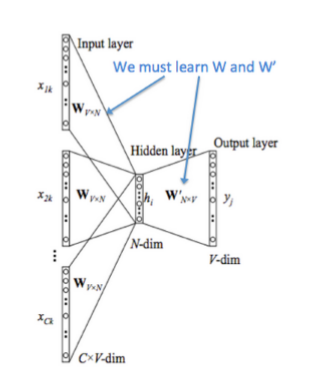
\includegraphics[width=0.4\textwidth]{Figures/CBOW.PNG}
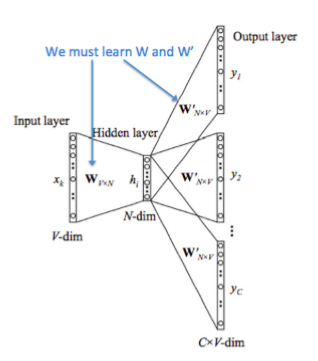
\includegraphics[width=0.4\textwidth]{Figures/SkipGram.PNG}
\caption{CBOW vs. SkipGram methods of training \footnotemark}
\end{center}
\end{figure}
\footnotetext{\url{http://cs224d.stanford.edu/lecture_notes/LectureNotes1.pdf}}

\paragraph{\wordtovec} \wordtovec \citep{Mikolov2013b} is a two-layer neural net that processes text. Its input is a text corpus and its output is a set of feature vectors for word types in that corpus. It treats words as distinct states and looks for the transitional probabilities between those states, i.e. the likelihood that they will co-occur. \wordtovec groups the vectors of similar words in vector space and can, thus, detect similarities mathematically. It does this by using the numerical representations of features such as the context of individual words to generate the word vectors. The model adjusts the vector components if it is unable to make accurate predictions of the word's context based on its assigned feature vector in the case of SkipGram (vice versa for CBOW). That is how the vectors of words judged to be similar based on their context are plotted closer together.

\wordtovec is widely used among the NLP research community to calculate the similarity of words. This can be applied to information retrieval tasks, for example, where it can be used to calculate the similarity between query vectors and their candidate documents \citep{Roy2018}.

\subsection{Character-level}
In a character-level embedding model, the vector for a word is constructed from the character n-grams that compose it. Since these are shared across words, these models can even generate embeddings for word they haven't encountered before. They also tend to handle infrequent words better, where word embedding models suffer from lack of sufficient training.

\paragraph{\fasttext}
\fasttext \citep{Bojanowski2017} is an adaptation of the \wordtovec model that seeks to enrich its word vectors with subword information. It composes a word vector by summing the n-gram vectors constituting the word. \fasttext supports training CBOW or Skip-gram models using negative sampling, softmax or hierarchical softmax loss functions. It also stores the positional information of these n-grams embedded in the resultant vector. For example, for the word \textit{clean}, with n = 2, the \fasttext representations for the character n-grams is \textit{$\langle$c,cl,le,ea,an,n$\rangle$}, where $\langle$ and $\rangle$ are boundary symbols to help distinguish between n-grams of a word and entire words. For example, the word \textit{an} would be represented as \textit{$\langle$an$\rangle$} to distinguish it from the identical n-gram \textit{an} observed in \textit{clean} and other such words. Inherently, this also allows you to capture meaning for suffixes/prefixes.
Therefore, the vector for the the word \textit{today} will not be the same as the vector for its misspelled variant \textit{tdoay} as the n-grams constituting both these vectors are very different.

\fasttext is widely used in text classification tasks like spam detection and sentiment analysis.

\subsection{Document-level}
Document-level embeddings are unsupervised methods for learning distributed representations of spans of text (sentences, paragraphs or documents). They are useful for generalisations as they concern themselves primarily with representing the semantics of the text \citep{Le2014}.
\paragraph{\doctovec}
Paragraph Vector (\doctovec) is an extension of \wordtovec that aims to learn how to project a document into a latent d-dimensional space regardless of its length. It works by taking context words and a paragraph ID as input and predicts a word central to a randomly sampled set of consecutive words from the paragraph \citep{Lau:Baldwin:2016b}. This is essentially the \wordtovec CBOW model that uses one extra vector to represent the paragraph ID, which is unique for each document (\figref{fig:d2vVSw2v}). Similarly, the \doctovec SkipGram model uses the paragraph vector to predict context words, or words that it expects to be observed in the document.
\begin{figure}[h!]
\begin{center}
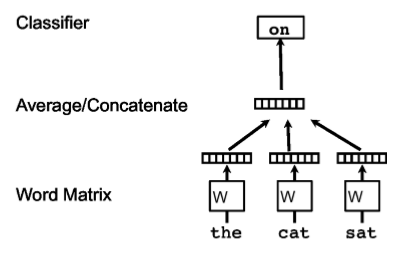
\includegraphics[width=0.4\textwidth]{Figures/w2vCBOW.PNG}
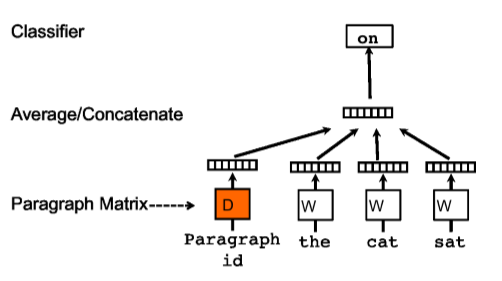
\includegraphics[width=0.4\textwidth]{Figures/d2vCBOW.PNG}
\caption{\wordtovec CBOW vs \doctovec CBOW models \citep{Le2014}}
\label{fig:d2vVSw2v}
\end{center}
\end{figure}
This paragraph vector is trained along with the word vector to hold a numerical representation of the document it identifies. This model, called \textit{Distributed Memory version of Paragraph Vector (PV-DM)} is actually faster (as opposed to \wordtovec word averaging) and consumes less memory, since it does not retain the individual word vectors.

\doctovec has been shown to work well in multi-class text classification and sentiment analysis problems.

\paragraph{\infersent}
\infersent \citep{Conneau2017} is a sentence embedding method trained on natural language inference data to provide semantic representations of English text. It uses the Stanford Natural Language Inference (SNLI) Corpus, a set of 570,000 pairs of sentences labelled one of 3 categories: neutral, contradiction and entailment, to train a classifier over a sentence encoder \figref{fig:inferSent}. Both the sentences of a pair are encoded using the same encoder, while the classifier is trained on the pair representation constructed from the two individual sentence embeddings. \cite{Conneau2017} adopt a bi-directional LSTM that encodes the sentences using a max-pooling operator.
\begin{figure}[h!]
\begin{center}
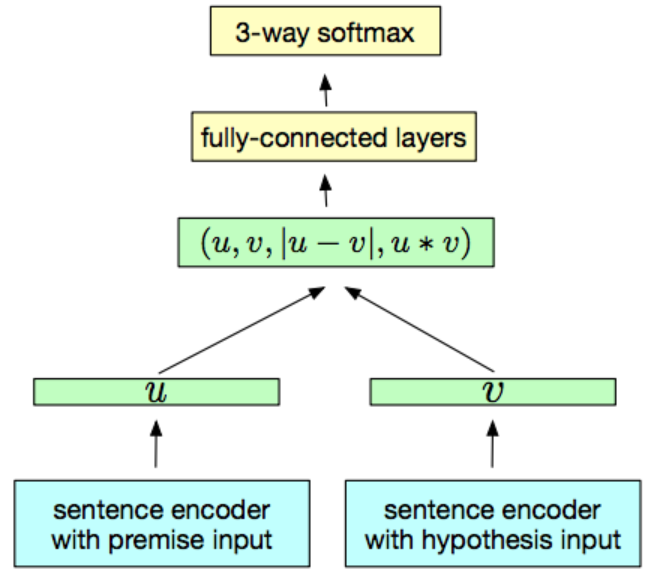
\includegraphics[width=0.5\textwidth]{Figures/InferSent.PNG}
\caption{The sentence encoder and classifier of \infersent \citep{Conneau2017}}
\label{fig:inferSent}
\end{center}
\end{figure}
\infersent has been shown to work well on transfer learning tasks-- a model that is trained to solve one task used to solve another \citep{Conneau2017}.

\subsection{Contextualised Embeddings}
The models so far exhibit one fundamental flaw-- they generate the same embedding for a word regardless of  its context. Consider again the word \textit{bridge} that displays polysemy and would be represented with the same vector embedding despite its difference in meaning in the following sentences:
\begin{enumerate}
\item \textit{The \underline{bridge} is under construction.}
\item \textit{I met John for a game of \underline{bridge}.}
\item \textit{We need to \underline{bridge} the gap between the rich and poor.}
\end{enumerate}

\noindent
Contextualised word embeddings aim to capture word semantics in different contexts to address the context-dependent nature of such words.

\paragraph{\elmo}
\elmo (Embeddings from Language Models) is an LSTM-based model that is trained on a corpus to generate a vector representation of a word using the hidden states of the LSTM \citep{Peters2018}. The language model is trained by reading the sentences both forward and backward, i.e. it learns to predict the next word given the past words, as well as the previous word given the future words-- effectively performing the task of two models. However, rather than using the embedding of the words from a word embedding matrix, each token is converted to an appropriate representation using character embeddings, which is then run through a convolutional layer using a number of filters, followed by a max-pool layer.The resultant representation is passed through a 2-layer highway network before being provided as the input to the LSTM layer.
There are a number of reasons for these transformations:
\begin{enumerate}
    \item Character embeddings are preferred because they are capable of picking up morphological features that word-level embeddings could miss.
    \item The convolution filters detect n-gram features that build more powerful representations.
    \item The highway network layers allow the information to be transferred more smoothly. 
\end{enumerate}

By using a multi-layer LSTM, which also considers the output sequence of the previous layer as input (in addition to the plain sequence of words), each layer of the model is able to learn a different characteristic of the language.

\elmo has been shown to work impressively well on tasks ranging from question-answering to sentiment analysis \citep{Peters2018}.

\paragraph{\bert}
Consider the sentence \textit{I need to make a bank deposit}. A left unidirectional contextual model would use the context words on the left of \textit{bank} (\textit{I, need, to, make, a}) to contextualise it and would leave out \textit{deposit}. A right unidirectional model would only use \textit{deposit} and leave out the rest. In either case, we may not be able to capture the word's context accurately. \elmo attempts to handle this by stacking a forward and backward LSTM.

As the name suggests, \bert (Bidirectional Encoder Representations from Transformers) uses birectional transformers to solve the same problem. A transformer is an encoder-decoder architecture model that uses attention mechanisms to project the whole sequence of text to the decoder at once rather than sequentially. They are preferred over conventional sequential models like LSTMs and RNNs because they model long term dependencies among tokens more effectively and eliminate the need for the sequential dependency on previous tokens. \bert models text by employing a technique known as \textit{masked language modelling} to mask 15\% of the words in a sentence and then forces itself to learn how to use their positional information to infer them. It does this because it utilises only the encoders from transformers, which would otherwise ``see'' all the words during the encoding phase.

\bert has been shown to work as well as \elmo on a range of tasks, including non-linguistic tasks like quantitative trading.

\paragraph{\flair}
\flair \citep{Akbik2018} is a sequence labeling architecture built on top of neural language modeling and trained without any explicit notion of words. Therefore, it models a word as a string of characters solely dependent on its contextual use, without regard for its meaning. It feeds a sentence as input into a pre-trained bidirectional character language model to retrieve a contextual embedding for each word in the sentence. The embedding is created by extracting the cell states for the first and last characters of the word. This word embedding is then passed into a bidrectional LSTM-CRF sequence labeller.

\begin{figure}[h!]
\begin{center}
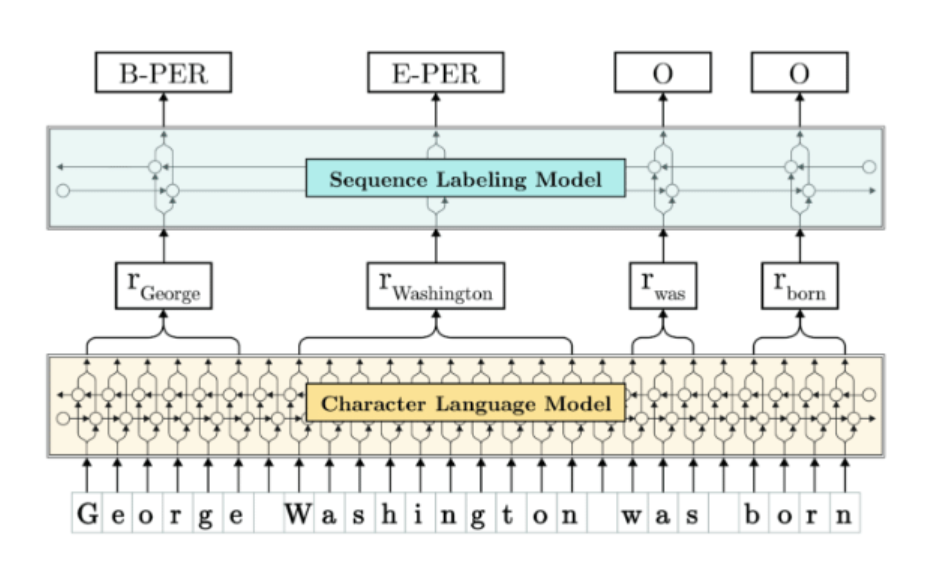
\includegraphics[width=0.8\textwidth]{Figures/Flair.PNG}
\caption{\flair performing NER tagging\footnotemark}
\label{fig:flair}
\end{center}
\end{figure}
\footnotetext{\url{https://research.zalando.com/welcome/mission/research-projects/flair-nlp/}}
\flair has been shown to outperfrom previous state-of-the-art embedding models in various downstream tasks like sequence labelling and named-entity recognition, as seen in \figref{fig:flair} \citep{Akbik2018}.

\section{Summary}
In this chapter, we provided a brief overview on multiword expressions and their importance. We discussed the prediction of the compositionality of such expressions and detailed some of the existing methods used in this task. Finally, we described some of the modern language embedding models and their use in natural language processing.

In the next chapter, we will employ the embedding models discussed to model the compositionality of MWEs and compare their performance.

%\section{Multi-task Learning}
%\label{sec:MTL}
%\cite{Kazuma2016},\cite{Coll2018}, \cite{Subramanian2018}, \cite{McCann2018}, \cite{Sanh2018}, \cite{Fares2018}, 
